\subsection{Vehicle}
The rover uses an Ackermann steering mechanism to be able to navigate. Unlike a manipulator, it is not a serial connection. Forward kinematics cannot be used on a mobile robot. Ackermann steering allows the front wheels to rotate independently, about a common center point. This center point is called the \textit{Instantaneous Center of Curvature} (ICC). In general, it uses a four bar linkage in a trapezoidal shape. However the Curiosity Mars Rover and the Sample-Return Rover does not use this linkage, but the model still holds. 

\begin{figure}[h!]
	\centering
	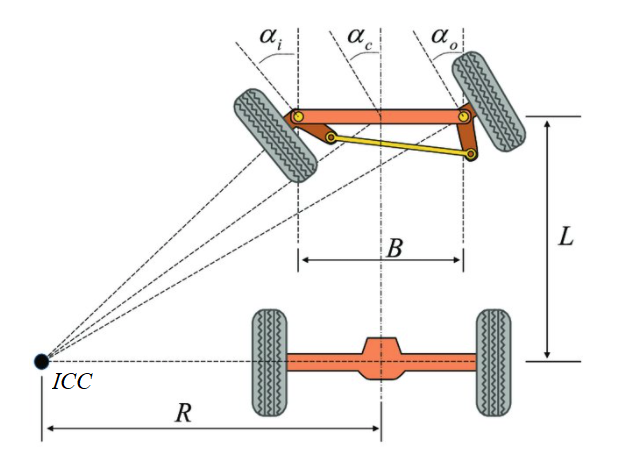
\includegraphics[scale=0.65]{sections/robot-design/images/ackermann_steering.png}
	\label{sample_return_rover:robot_design:ackermann}
	\caption{Diagram for Ackermann Steering}
\end{figure}

\subsection{Arm}
In robotics, forward kinematics is used to find the position and orientation of the robot's end-effector (or gripper) given the joint angles. In this course, joints can have two different types: \textit{revolute} and \textit{prismatic}. A revolute joint rotates about an axis. A prismatic joint translates linearly along an an axis. A robotic arm can be considered as serial kinematic chains, because starting from the base of the arm the rest of the joints and links position are dependent on its parent joint and link orientation. Each joint can be assigned a coordinate frame with an x, y, and z axis. These frames represent either rotations or translation at a joint it is assigned to. These frames and their rotations/translation can be represented with a 3x3 matrix, which can then be put in a homogeneous transformation matrix and chained together to find the position of the end-effector. \\

The robot arm itself has 4 degrees of freedom, with it all being revolute. However, there are 8 frames in total, because 4 dummy frames are for Gazebo to properly render in the arm. The frames are shown in Figure~\ref{sample_return_rover:robot_design:arm_frames}. Its corresponding DH table is shown in Figure~\ref{table:2}. A list of the links are shown in Figure~\ref{sample_return_rover:robot_design:arm_diagram}. The links LeftFinger and RightFinger are just there for Gazebo to be able to rotate the end-effector fingers, but they are not used in the DH parameters and table.
\begin{figure}[H]
	\centering
	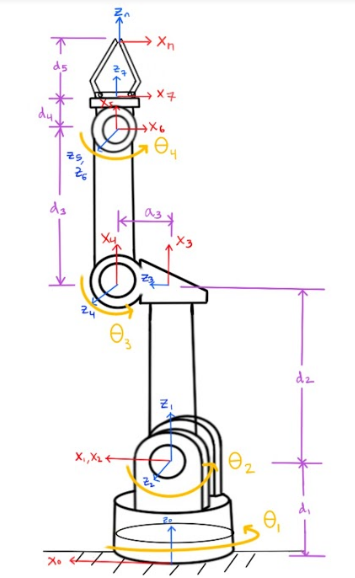
\includegraphics[scale=0.6]{sections/robot-design/images/arm_frames.png}
	\label{sample_return_rover:robot_design:arm_frames}
	\caption{DH Frames of the Arm}
\end{figure}

\begin{table}[H]
	\begin{center}
		\begin{tabular}{|c|c|c|c|c|} 
			\hline
			\textit{Link i} & \textit{$\theta$} & \textit{d} & \textit{$\alpha$} & \textit{a}\\
			\hline
			1 & $\theta_{1}$ & $d_{1}$ & 0 & 0 \\
			2 & 0 & 0 & -90 & 0 \\
			3 & $\theta_{2}$ - 90  & 0 & -90 & $d_{2}$ \\
			4 & 0  & $a_{3}$ & 90 & 0 \\ 
			5 & $\theta_{3}$ & 0 & 0 & $d_{3}$ \\
			6 & $\theta_{4}$ - 90 & 0 & -90 & 0 \\
			7 & 0 & $d_{4}$ & 0 & 0 \\
			n & 0 & $d_{5}$ & 0 & 0 \\
			\hline
		\end{tabular}
		\caption{\label{table:2} DH Table for the Arm }
	\end{center}
\end{table}

\begin{figure}[H]
	\centering
	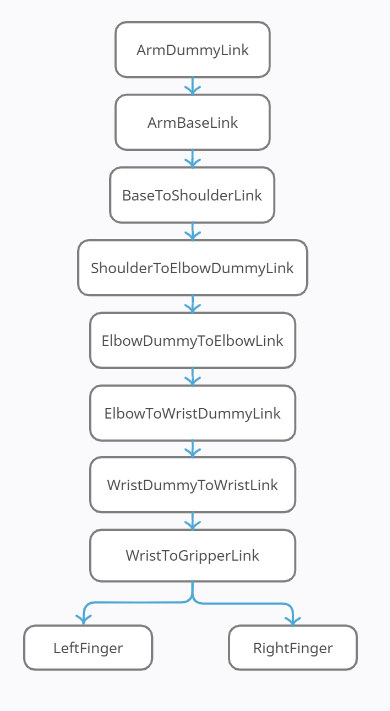
\includegraphics[scale=1.2]{sections/robot-design/images/arm_link_diagram.png}
	\label{sample_return_rover:robot_design:arm_diagram}
	\caption{Flowchart of the Arm Links}
\end{figure}
\newpage
To start calculating the forward kinematics, rotation matrices can be made for the frames. The basic rotation matrix for a rotation about the z-axis with an angle $\theta$ can be shown in Equation~\ref{sample_return_rover:fwd_kinematics:rz}. Using the DH Table, the homogeneous transformation matrices can now be written. The setup for this matrix is seen in Equation~\ref{sample_return_rover:fwd_kinematics:H0n}.

\begin{equation}
	R_{z, \theta} = \left[\begin{array}{ccc}
		cos(\theta) & sin(\theta) & 0 \\
		sin(\theta) & cos(\theta) & 0 \\
		0 & 0 & 1 \\
	\end{array}\right]
\label{sample_return_rover:fwd_kinematics:rz}	
\end{equation}

\begin{equation}
	H^{0}_{n} = \left[\begin{array}{cc}
		R^{0}_{n} & d^{0}_{n} \\
	    0 & 1 \\
	\end{array}\right]
\label{sample_return_rover:fwd_kinematics:H0n}
\end{equation} \\

To find the position and orientation of the end effector by using the homogeneous transformation matrices the distances between each frame needs to be defined. Table~\ref{table:3} defines all the lengths needed between the frames in regards to the CAD model.


\begin{table}[H]
	\begin{center}
		\begin{tabular}{|c|c|} 
			\hline 
			\textit{Distance between Frames} & \textit{Length} \\
			\hline
			Base to Frame 1 ($d_{1}$) & 2.9in \\
			Frame 2 to Frame 3 ($d_{2}$) & 7.73in \\
			Frame 3 to Frame 4 ($a_{3}$) & 1.76in \\
			Frame 4 to Frame 5 ($d_{3}$) & 8.93in \\
			Frame 6 to Frame 7 ($d_{4}$) & 1in \\
			Frame 7 to Frame n ($d_{5}$) & 1.41in \\
			\hline
		\end{tabular}
		\caption{\label{table:3}Table of Link Lengths of the Arm}
	\end{center}
\end{table}

Note that the arm's home position starts with all angles being at 0, so the arm is fully upward. Each joint has a limit for its range of motion so that the robot does not crash into itself. This can be seen in Equations~\ref{th1} - \ref{th4}. \\
\begin{equation}
	\theta_{1} = [-\pi,\; + \pi]
	\label{th1} 
\end{equation}

\begin{equation}
	\theta_{2} = \left[\begin{array}{c}
		0,\; +\frac{2\pi}{3} \\
	\end{array}\right] 
	\label{th2}
\end{equation}

\begin{equation}
	\theta_{3} = [0,\; + \pi]
	\label{th3} 
\end{equation}	

\begin{equation}
	\theta_{4} = \left[\begin{array}{c}
		-\frac{2\pi}{3},\; +\frac{2\pi}{3} \\
	\end{array}\right] 
\label{th4}
\end{equation}
\newpage
The final homogeneous matrix can be also written as Equation~\ref{sample_return_rover:fwd_kinematics:H0n_2}: 

\begin{equation}
	H^{0}_{n} = \left[\begin{array}{ccc}
		x^{0}_{n} & y^{0}_{n} & z^{0}_{n}\\
	\end{array}\right]
	\label{sample_return_rover:fwd_kinematics:H0n_2}
\end{equation}
where
\begin{equation}
	x^{0}_{n} = c_{1}\left[\begin{array}{c} d_{2}s_{2}+a_{2}c_{2}+d_{3}s_{23}+(d_{4}+d_{5})s_{234}\\
	\end{array}\right]
	\label{sample_return_rover:fwd_kinematics:x0n}
\end{equation}
\begin{equation}
	y^{0}_{n} = s_{1}\left[\begin{array}{c}
		d_{2}s_{2}+a_{2}c_{2}+d_{3}s_{23}+(d_{4}+d_{5})s_{234}\\
	\end{array}\right]
	\label{sample_return_rover:fwd_kinematics:y0n}
\end{equation}

\begin{equation}
	z^{0}_{n} = \left[\begin{array}{c}
		d_{1}+d_{2}c_{2}-a_{2}s_{2}+d_{3}c_{23}+(d_{4}+d_{5})c_{234}\\
	\end{array}\right]
	\label{sample_return_rover:fwd_kinematics:z0n}
\end{equation}

Note that c is cos, s is sin, and multiple numbered subscripts means they are added together. For example, $s_{23}$ is equivalent to (sin(${\theta_{2}}$) + sin(${\theta_{3}}$)).
